\section{Approach}
\label{sec:approach}
SEP events are comprised of high energy particles such as protons, electrons and alpha particles, with protons being the highest risk to space and ground based infrastructure \cite{wilkinson1991tdrs}.
At 1 AU, relativistic electrons experience less scattering than protons when traveling to earth. Because of this, an early wanring forecast model can be created that only uses preceding
relativistc electrons to warn us of high energy protons \cite{posner2007forecasting}, \cite{torres2025machine}.  A time series of raw particle channels from COSTEP is used for forecasting using time series transformers.
We build a series of transformer models with different encoding architectures that captures the correlation of proton and electron intensity
using multiple methods.

In Section \ref{sec:input} we discuss the particle time series and the instrument. Section \ref{sec:transformer} provides an explantion of what transformers are and they differ
to previous machine learning models. \ref{sec:positionalencodingmethods} justifies the chosen positional encodings architectures.

\subsection{Input}
\label{sec:input}

\begin{figure}[!htbp]
    \centering
    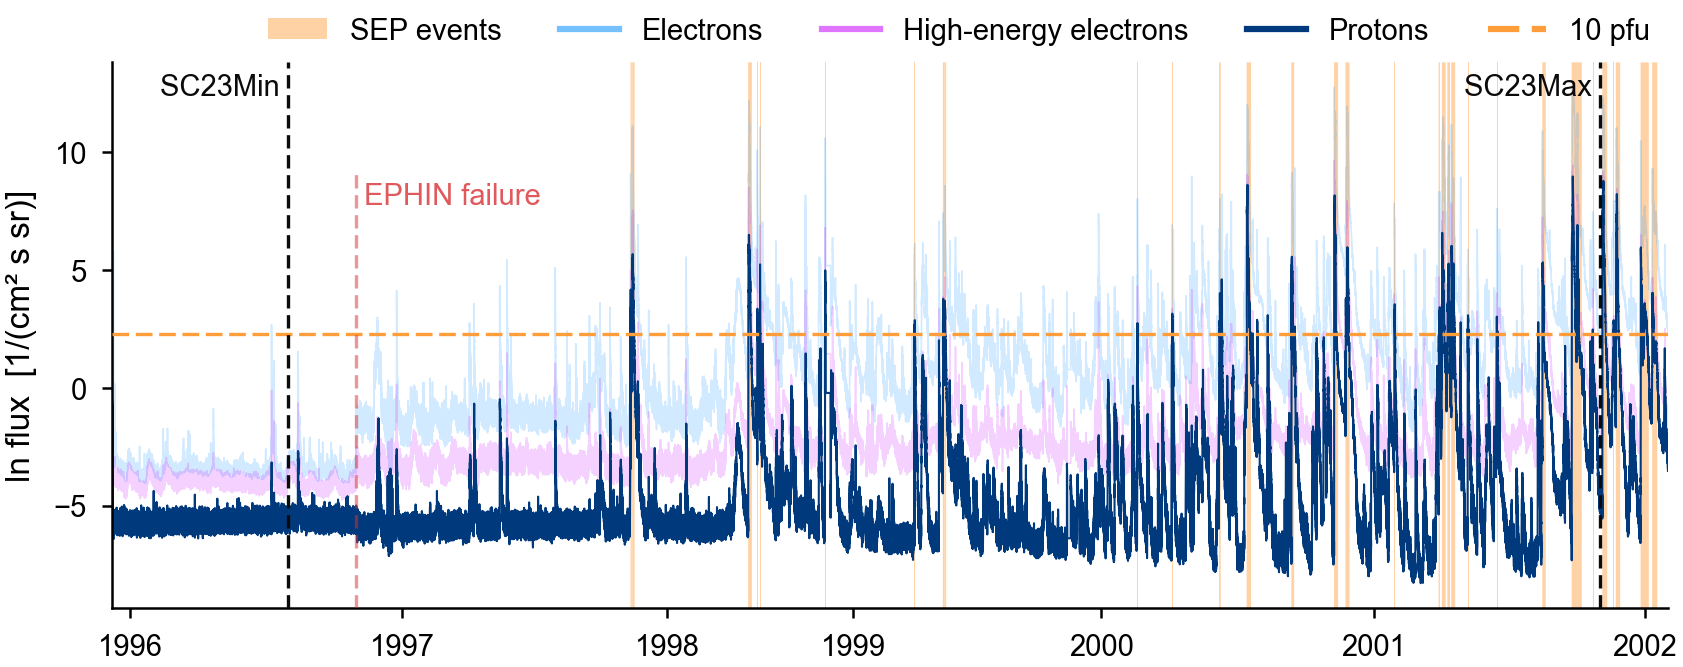
\includegraphics[width=\textwidth]{figs/approach/input/flux_series.png}
    \caption{SOHO COSTEP-EPHIN dataset from 1995-2002}
    \label{fig:data_overview_single}
\end{figure}

The particle channel data are obtained from the Comprehensive Suprathermal and Energetic Particle Analyzer - Electron Proton Helium Instrument (COSTEP-EPHIN)  on the Solar and Heliospheric Observatory (SOHO). SOHO first launched on December 2nd 1995 to take in situ of energy depostion and particle acceleration in the solar atmosphere \cite{SOHOCOSTEPEPHINCDFPT1M}.
SOHO orbits between the earth and sun around Lagrange Point 1 (L1), which is approximately 1.5 million kilometers from earth. L1 is an ideal location 
for space weather isntrumetns as any satelltie situatued there enjoys an uninteruppted view of the sun.
The EPHIN instirments switched to failure mode that reduced the energy ranges it was able to read on October of 1996 \cite{kuhl2019revising}.
\cite{torres2025machine} provides a dataset of 39 SEP identified events using the particle data recorded by COSTEP-EPHIN. Two relatavistic electron intensities channels $\geq$0.25 and $\geq$0.67 MeV \cite{mullermellin1995costep} are the precursors for our incoming protons. Proton channels are seperated into four energy channels (P4,P8,P25, P41) each corresponding to  different energy ranges.
Proton channel P4 corresponds to the energy range $4.3 - 7.8 \text{ MeV}$, P8 corresponds with $7.8-25 - 7.8 \text{ MeV}$,  P25 corresponds with  $25 - 40.9 \text{ MeV}$, and P41 corresponds with $40.9 - 53 - 7.8 \text{ MeV}$. To retreive a $>10$ MeV proton flux channel, a sum of the energy integrated fluxes P8,P25, and P41 channels minus the range
$7.8-10$ MeV is performed. The latter channel is determined by the a power law spectrum  interpolation of the first two channels, P4 and P8, differential fluxes and their mean energies \cite{torres2025machine}.

SEP events were then identified for storms larger than 10 proton flux unit (pfu). Each event is partitioned into phases to highlight definable features: Onset, Threhsold, Peak, End.
The onset is defined when the flux rises three times the error bar above the pre-event background, the threshold is when the flux first crosses over 10 pfu and the end time is when it drops again below 2 pfu.\cite{torres2025machine}.

\subsection{Why Transformers}
the computaitonal power of a transfomrer can be parelized requireing less operaitons. Long range dependencies can be handled much easier
with larger winow lengths. Inputs  passes forward and back signals that help to make predictions.
As the input window length grows, the harder it is to learn long range dpeendencies on RNN and NN modles \cite{zhao2026transformersurvey}. Self Attention could yield more interpretabhle models \cite{vaswani2017attention}.
NN and RNN scale suboptimally to large datasets compared to transformer models \cite{zhao2026transformersurvey}

Physics based models simulating particle accelration and trnasport processes are omputionatially expensive and with the limited amount of data limited \cite{Camporeale2019} \cite{yu2026} \cite{kasapis2026review}.
Fruthermore lmiations in forecast timeliness forces a trade off with realism \cite{yu2026}.

\subsection{Transformers}
\label{sec:transformer}

The original transformer is comprised of encoder-decoder stacks with built in self attention modules that translates inputs $\mathbf{X}$ into vectors $\mathbf{Z}$,
identifies correlations and relationships, and outputs a sequence of predictions $\mathbf{Y}$. The encoder stack handles the $\mathbf{X \rightarrow Z}$ transformations while the decoder  handles $\mathbf{Z \rightarrow Y}$ \cite{vaswani2017attention}.
Because we are only predicting a singular timestamp of proton flux in the future, we drop our decoder stacks as its purpose is to gneerate a sequence of 
outputs from $\mathbf{Y}$ rather than one value \cite{vaswani2017attention}.

For our time series data, we use two hours of historical particle flux data of our two electron channels and $>10$ MeV proton channel. The magnitude in differences of fluxes between our channels  is large enough to cause 
unstable trianing and testing therefore we apply a natural $\log$ transformation to the entire dataset, resulting compressing the mean and  variance on the same scale. The standard method is to 
subtract by the mean and divide by the standard deviation, a process called "standardization". To ensure our NN and RNN
align with \cite{torres2025machine} model results, the prior method is selected instead to replicate \cite{torres2025machine}

We set $t$ to indicate present time. Becasue of the cadence of 5 minutes,
 $t - 25$ timestamps creates twenty-four 5-min intervals of particle flux forming a window of inputs before and including the current time. For each window, we define an input sample:
$$
\mathbf{X} \in \mathbb{R}^{l \times v} = \mathbb{R}^{25 \times 3}
$$
where $l$ is the length of the input window and $v$ is the number of variates. A processes that translates our particle fluxes at each timestep into transformer
readable vecotrs, embedding, is calculated by:
$$
\mathbf{
U} = \mathbf{XW_p}^T + \mathbf{1b_p}^T, \mathbf{1} \in \mathbb{R}^{l \times 1}
$$
$\mathbf{W_p} \in \mathbb{R}^{d \times v}$ and $\mathbf{b_p} \in \mathbb{R}^{d}$ are weighted and bias vectors respectively. They are initialized randomly at the start of training and then used to compute $\mathbf{U} \in \mathbb{R}^{l \times d}$.
After every training cycle, these vectors  updates and learn to optimize minimizing loss, error.
$d$  is the dimension of the embedding vector that represents our inputs. For large $d$, inputs are characterized at a higher resoltution allowing  models to learn finer grain patterns at the cost of compuational power and risk of overfitting. 
The number of parameters in a model is proportional to the size of $\mathbf{W_p}$ and $\mathbf{b_p}$ \cite{vaswani2017attention} \cite{zerveas2020transformer}

\begin{table}[!htbp]
\centering
\caption{Total number of trainable parameters for each model.}
\label{tab:param-count}
\begin{tabular}{l r}
\toprule
Model & Parameters \\
\midrule
NN          & 2,311 \\
RNN         & 3,181 \\
\midrule
Sinusoidal  & 3,361 \\
Zero-Init   & 3,761 \\
RoPE        & 3,361 \\
\bottomrule
\end{tabular}
\end{table}


To match parameter size of \cite{torres2025machine} we use $d = 16$. Our transformer models are slighlty larger than the RNN and NN provided by \cite{torres2025machine}. A model size $d=8$ would 
greatly reduce the models far below the parameter count of RNN and NN.  Table \ref{tab:param-count} provides
a count of all parameters in each machin learning model in this study.
The RNN and NN are implemented  with two layers: One layer is hidden with 30 units and then a second dense single output layer.
The RNN is comprised of  Gated Recurrent Units (GRU) for its  hidden layers while the NN uses hidden layers.
The NN model uses the same three channels for 25 timestep intervals.
The RNN  has the 30 GRU units plus our three channel input \cite{torres2025machine}. 
All models (RNN,NN, transformers) minimize the loss function with mean square error during training.
\begin{figure}[H]
    \centering
    \resizebox{0.6\textwidth}{!}{
    \begin{tikzpicture}[
        pebox/.style={
            draw, rounded corners=2pt, fill=green!25,
            minimum width=2cm, minimum height=1cm, thick,
        },
        mhbox/.style={
            draw, rounded corners=2pt, fill=red!25,
            minimum width=3cm, minimum height=1.5cm, thick,
        },
        normbox/.style={
            draw, rounded corners=2pt, fill=orange!25,
            minimum width=3.0cm, minimum height=.5cm, thick,
        },
        feedforwardbox/.style={
            draw, rounded corners=2pt, fill=violet!25,
            minimum width=3.0cm, minimum height=1.5cm, thick,
        },
        linearbox/.style={
            draw, rounded corners=2pt, fill=yellow!25,
            minimum width=3.5cm, minimum height=.5cm, thick,
        },
        softmaxbox/.style={
            draw, rounded corners=2pt, fill=teal!25,
            minimum width=3.5cm, minimum height=.5cm, thick,
        },
        scale = 1
    ]

        % outer container: the whole encoder block


        \node (pe) at (0,-8) {$\bigoplus$};
        \node[
            draw,
            rounded corners=15pt,
            fill=gray!25,
            minimum width=6cm,
            minimum height=8.5cm,
            thick,
            above = 20mm of pe,
        ] (outer){};

        % positional-encoding options, stacked left of pe: RoPE level with pe,
        % Sinusoidal/Zero-Init symmetric above/below it -- no manual coordinates
        
        \node[text= olive, text width = 3 cm, align=center](pe_disclaimer) at (-6,-6){Only one of the positoinal enoders (RoPE, Sin, Zero) are used for each training run };
        \node[pebox, above left =.5mm and 2cm of pe] (Sinusoidal) {Sinusoidal};
        \node[pebox, below left =.5mm and 2cm of pe] (Zero-Init) {Zero-Init};
        \node[mhbox, above=35mm of pe, text width = 2 cm, align=center] (MultiHead) {Multi-Head Attention};
        \node[normbox, above = 1.5 cm of MultiHead] (norm1){Norm};
        \node[pebox, left=2cm of MultiHead] (RoPE) {RoPE};
        \node[
            draw, rounded corners=5pt, fill=blue!25,
            minimum width=2cm, minimum height=1cm, thick,
            below=10mm of pe,
        ] (Input_Embedding) {Input Embedding};
        \node[feedforwardbox, above =  5mm of norm1, text width = 2 cm, align=center](FeedForward){Feed Forward};
        \node[below= 1cm of Input_Embedding, text width = 3cm, align=center](input) {2 hour window of high and low electrons w/ current proton flux};
        \node[normbox, below = 2cm of MultiHead](norm2){Norm};


        \node[align = center] at (-5,-2){$\times 1$ Encoding Layers};
        \node[above = 5mm of MultiHead] (pe2) {$\bigoplus$};
        \node[above = 5mm of FeedForward] (pe3) {$\bigoplus$};
        \node (pe) at (0,-8) {$\bigoplus$};
        \node[linearbox, above = 8mm of pe3](linear){Linear};

        \draw[->,thick](input.north) -- (Input_Embedding.south);
        \draw[->, thick, rounded corners=5pt] (Input_Embedding.north) -- (pe.south);
        \draw[->, thick, rounded corners=5pt] (RoPE.east) -- (MultiHead.west);
        \draw[->, thick, rounded corners=5pt] (Zero-Init.east) -| ++(5mm,8.55mm) -- (pe.west);
        \draw[->, thick, rounded corners=5pt] (Sinusoidal.east) -| ++(5mm,-8.55mm) -- (pe.west);
        \draw[->, thick, rounded corners=5pt] (pe.east) -| ++(15mm,0) |- (pe2.east);
        \draw[->, thick, rounded corners=5pt] (pe2.east) -| ++(15mm,0) |- (pe3.east);
        \draw[->, thick, rounded corners=5pt] (norm2.north) |- ++(-7mm,15mm) -| ($(MultiHead.south west) + (5mm,0)$);
        \draw[->, thick, rounded corners=5pt] (norm2.north) |- ++(7mm,15mm) -| ($(MultiHead.south east) - (5mm,0)$);
        \draw[->, thick] (norm2.north)  -- (MultiHead.south);
        \draw[->, thick] (pe.north)  -- (norm2.south);
        \draw[->,thick](norm1.north) -- (FeedForward.south);
        \draw[->,thick](FeedForward.north) -- (pe3.south);
        \draw[->, thick](pe3.north) -- (linear.south);
        \draw[->, thick , rounded corners=5pt]($(pe)!0.60!(MultiHead)$) -| ++(-25mm, 15mm) |- (norm1.west);
        \draw[->,thick](MultiHead.north)--(pe2.south);
        \draw[->, thick](pe2.north)--(norm1.south);
        \draw[->,thick, text width = 3 cm, align=center](linear.north) -- ++(0,5mm) node[above] {Forecasted proton flux at $t+6$/$t+12$};
        \path (5,-2); % invisible point, balances the bounding box against the "$\times 1$" label on the left
    \end{tikzpicture}
    }
    \caption{Generic transformer architecture where positional encoding methods are indicated to show the difference between all models}
    
    \label{fig:transformer-pe}
\end{figure}


\subsection{Positional Encoding Methods}
\label{sec:positionalencodingmethods}

Transformer models computes updates in $\mathbf{W_p}$ and $\mathbf{b_p}$ in parallel. This allows for large input sequences
to be read at the same time without "forgetting" related timestamps that are far apart from eachother in the window.  
Any reshuffling of the vectors that make  up $\mathbf{U}$ has no effect on the the update calculation. 
Additional positional information must be injected to bring  context to our input window \cite{vaswani2017attention}.
For all input vectors $\mathbf{u_w}$ we add a $\mathbf{w_{\text{pos}, w}}$:
$$
\mathbf{U' = U + W_{\text{pos}}} , \mathbf{W_\text{pos}} \in \mathbb{R}^{l \times d}
$$
RNNs and NNs in contrast, reads the inputs sequentially learning order inherently.

The particle flux dataset is small, therefore different positional encoding (PE) could effect predictions.
PE is said to be a major factor in "length generalization", ability to extrapolate effectively  large sequences of events
from smaller training context windows. Transformers without PE outperform those with explicit PE methods \cite{kazemnejad2023impact}. 


\subsubsection{Sinusoidal Positional Encoding}
\label{sec:sinusoidalPE}
Sinusoidal positional encoding was first introduced in the original proposed transformer architecture paper \cite{vaswani2017attention}.
It is an absolute position encoding method that uses sinusoidal and cosine functions of different frequencies to encode the positional indexes of tokens in a sequence.
The input window is split into smaller chunks called tokens. For each token, a vector of dimension, $d$ is generated. The vector is determined by the position, $pos$, in the window and the length of the vector, $d$.
$i$ is the dimension of the PE vector. Odd and even indexes in the vector are determined by \eqref{cosPE} and \eqref{sinPE} respectively. This gives us a new vector $\mathbf{w_\text{pos}} \in \mathbb{R}^{l \times 1}$.
\eqref{sinPE} and \eqref{cosPE} to represent a linear relationship between two encoded positions.

\begin{equation}
    \label{sinPE}
    PE_{(pos,2i)} = \sin (pos / 10000^{2i/d})
\end{equation}


\begin{equation}
    \label{cosPE}
    PE_{(pos,2i+1)} = \cos(pos/10000^{2i/d})
\end{equation}


 The frequency decreases exponentially by a scale factor as the position in the model dimensions increase.
 Similarly stated in Section \ref{sec:transformer}, in the short term we can map small patterns in data, a $\sin/\cos$ function with a high frequency.
 At large vector indexes the frequency greatly decreases, taking on a more linear relationship.
 The positions are encoded uniquely based on value and position, allowing it to scale to unlimited sequence lengths. \cite{vaswani2017attention}

\subsubsection{Rotary Positional Embedding}

Rotary Positional Embedding (RoPE) is a PE method that stores the poistion infomration of a token,$m$ in a squence
in the total rotation of that query-key vectors by some angle $\theta_i$. The rotation amount is calculated by:
$$
\theta_i = 10000^{-2(i-1)/d}, \left\{i \in \mathbb{Z} \Bigg| 1 \leq i \leq \frac{d}{2}\right\}
$$
The rotation matrix is then applied to the token:
$$
r_{\theta_i} =  
\begin{bmatrix} 
\cos (m\theta_i) & -\sin (m\theta_i)  \\
\sin (m\theta_i) & \cos (m\theta_i )
\end{bmatrix}
$$
To generalize we stack our rotation values $\Theta = [\theta_1, ..., \theta_{d/2}]$ form the rotary matrix:

\begin{equation}
\mathbf{R}^{d}_{\Theta,m} =
\begin{pmatrix}
r_{\theta_1} & \mathbf{0} & \cdots & \mathbf{0} \\
\mathbf{0} & r_{\theta_2} & \cdots & \mathbf{0} \\
\vdots & \vdots & \ddots & \vdots \\
\mathbf{0} & \mathbf{0} & \cdots & r_{\theta_{d/2}}
\end{pmatrix}
= \operatorname{diag}\!\left(r_{\theta_1}, r_{\theta_2}, \dots, r_{\theta_{d/2}}\right)
\end{equation}
where each $\mathbf{0}$ is a $2 \times 2$ block of zeros, so $\mathbf{R}^{d}_{\Theta,m} \in \mathbb{R}^{d \times d}$.

Unlike Section \ref{sec:sinusoidalPE} and Section \ref{sec:ZeroPE}, the transformations are applied
directly to the self attention block as illustrated in \ref{fig:transformer-pe}, see Section \ref{sec:self-attention}.
The attention weight between two query-key in a sequence, $\mathbf{q}_m^T \mathbf{k}_n$, where $n$ is the position of the key vector,
is:
\begin{equation}
    \mathbf{q}_m^T \mathbf{k}_n = \mathbf{x}^T\mathbf{W}_q\mathbf{R}_{\Theta, n-m}^d \mathbf{W}_k\mathbf{x}_n
\end{equation}
where $ \mathbf{R}_{\Theta, n-m}^d = (\mathbf{R}_{\Theta, m}^d)^T \mathbf{R}_{\Theta, n}^d$.

A property of RoPE is long term decay.
This means that pairs of query-key at large relative distance will have less connection than those that are close to each other \cite{su2021roformer}.
For our flux data, this would coincide with the idea from \cite{posner2007forecasting} that only a short term forecasting of relativistic electrons is required to accurately predict future proton storms from 30 minutes to an hour. 

\subsubsection{Zero-Initialized}
\label{sec:ZeroPE}
Zero-Initialized positional encoding is another absolute positional that sets all  positional encoding parameters in a transformer to zero at the start of training. Positions of a timestamped flux has equal effects on each other at the start. As training continues, near timestamped fluxes learn to correlate to each other rather than further ones.
Zero init contrast Sinusoidal who all have non zero starting weight values.
This makes it reliable for generalization which is ideal for SEP data made almost entirely of background fluxes \cite{torres2025machine}.
Small near zero initializations sampled with normal distributions were found to perform better than larger ones \cite{ito2024learning}.

Most timestamps in the relatively small proton electron flux dataset are near zero background values.
A larger starting weights already has background information included leading to forecasting more background in the future during the early portion of training.
Its not until after rounds of epochs the model unlearns patterns to map rising phases in fluxes occur to make accurate predictions.

% \subsection{Auto-Gluon}
% Recurrent Neural Networks (RNN)s are unreliable for long range forecasting and irregular patterns \cite{zhao2026transformersurvey}.
% This is prevalent in our particle flux data with long periods of noise with sudden flux spikes when a storm occurs.
% The transformer architecture allows for capturing long patterns of behavior with improved predictions with parallel processing while RNNs process only in series.
% The Transformer attention mechanism is able to analyze all time steps at once and focus on relevant steps regardless of order \cite{vaswani2017attention}.
% This method of parallel analytical processing reveals subtle patterns that would be overlooked by RNNs \cite{zhao2026transformersurvey}.
% Our transformer will only have an encoding only architecture as we are forecasting one value of proton flux, therefore a single output layer is required only.
% If we were to predict a series proton fluxes then a decoder would be required.


\subsection{Self-Attention}
After computing our new input vectors with added PE, it can be fed into our multihead attention block.
To do this we first have to define our $QKV$ matrices. Randomly initialized weighted matrices $W_i^{QKV} \in \mathbb{R}^{d \times d_k}$ are procured.
$d_k  =d/h$ where $h$ is the number of heads. Our $QKV$ matrices are therefore:

\begin{align*}
    Q = U'W_i^Q\\
    K = U' W_i^K\\
    V = U'W_i^V
\end{align*}

where $i$ is the index of the head. For Multihead:
$$
\text{MultiHead}(Q,K,V) = \text{Concat}(\text{head}_i)W^O
$$
and
$$
\text{head}_i = \text{softmax}\left(\frac{Q^TK}{\sqrt{d_k}}\right)V
$$
$W^O$ is the output ptojection of the attention layer.
\label{sec:self-attention}

\subsection{Statistical and Empirical Models}
\label{sec: baseline_methods_used_for_comparison}
A persistent model as a baseline is included in our study. its a simple nowcast model in which the predicted proton flux value is the current proton flux value.
\cite{posner2007forecasting} Forecasting matrix will be compared to as well across the same metrics.

A multi variant linear regression model that reads in  our three channels of particle fluxes will also be used as a baseline for our transformer.
